\chapter{Model automobilu}
\label{sec:CarModel}\

V této kapitole je popsán model automobilu a jeho jednotlivé části.

Model automobilu je založen na platformě Alamak, která má
\textbf{2 servomotory} pro otáčení předních kol a
\textbf{2 PWM motory} pro řízení každého
zadního kola.

\textbf{Platforma Alamak} je řízená pomocí \textbf{NXP Freedom K66F}\cite{frdmk66UserGuide} spolu
s modulem \textbf{POLI-TFC} přípojeným do GPIO pinů MCU.
Detailní popis MCU a modulu jsou v podkapitolách \ref{sec:FRDM-K66F}
a \ref{sec:POLI-TFC}.

Pro komunikaci s platformou Alamak je použit \textbf{WiFi Access Point}, který je připojen k MCU
pomocí Ethernet portu.

\textbf{Řádková kamera}, která umístěna v přední části platformy,
se používá pro získání obrazu drahy.

Vše je napojeno pomocí baterie typu \textbf{NiMH} o napětí 7.2V.

Celý model je zobrazen na obrázku \ref{fig:car}.
\begin{figure}[h]
    \centering
    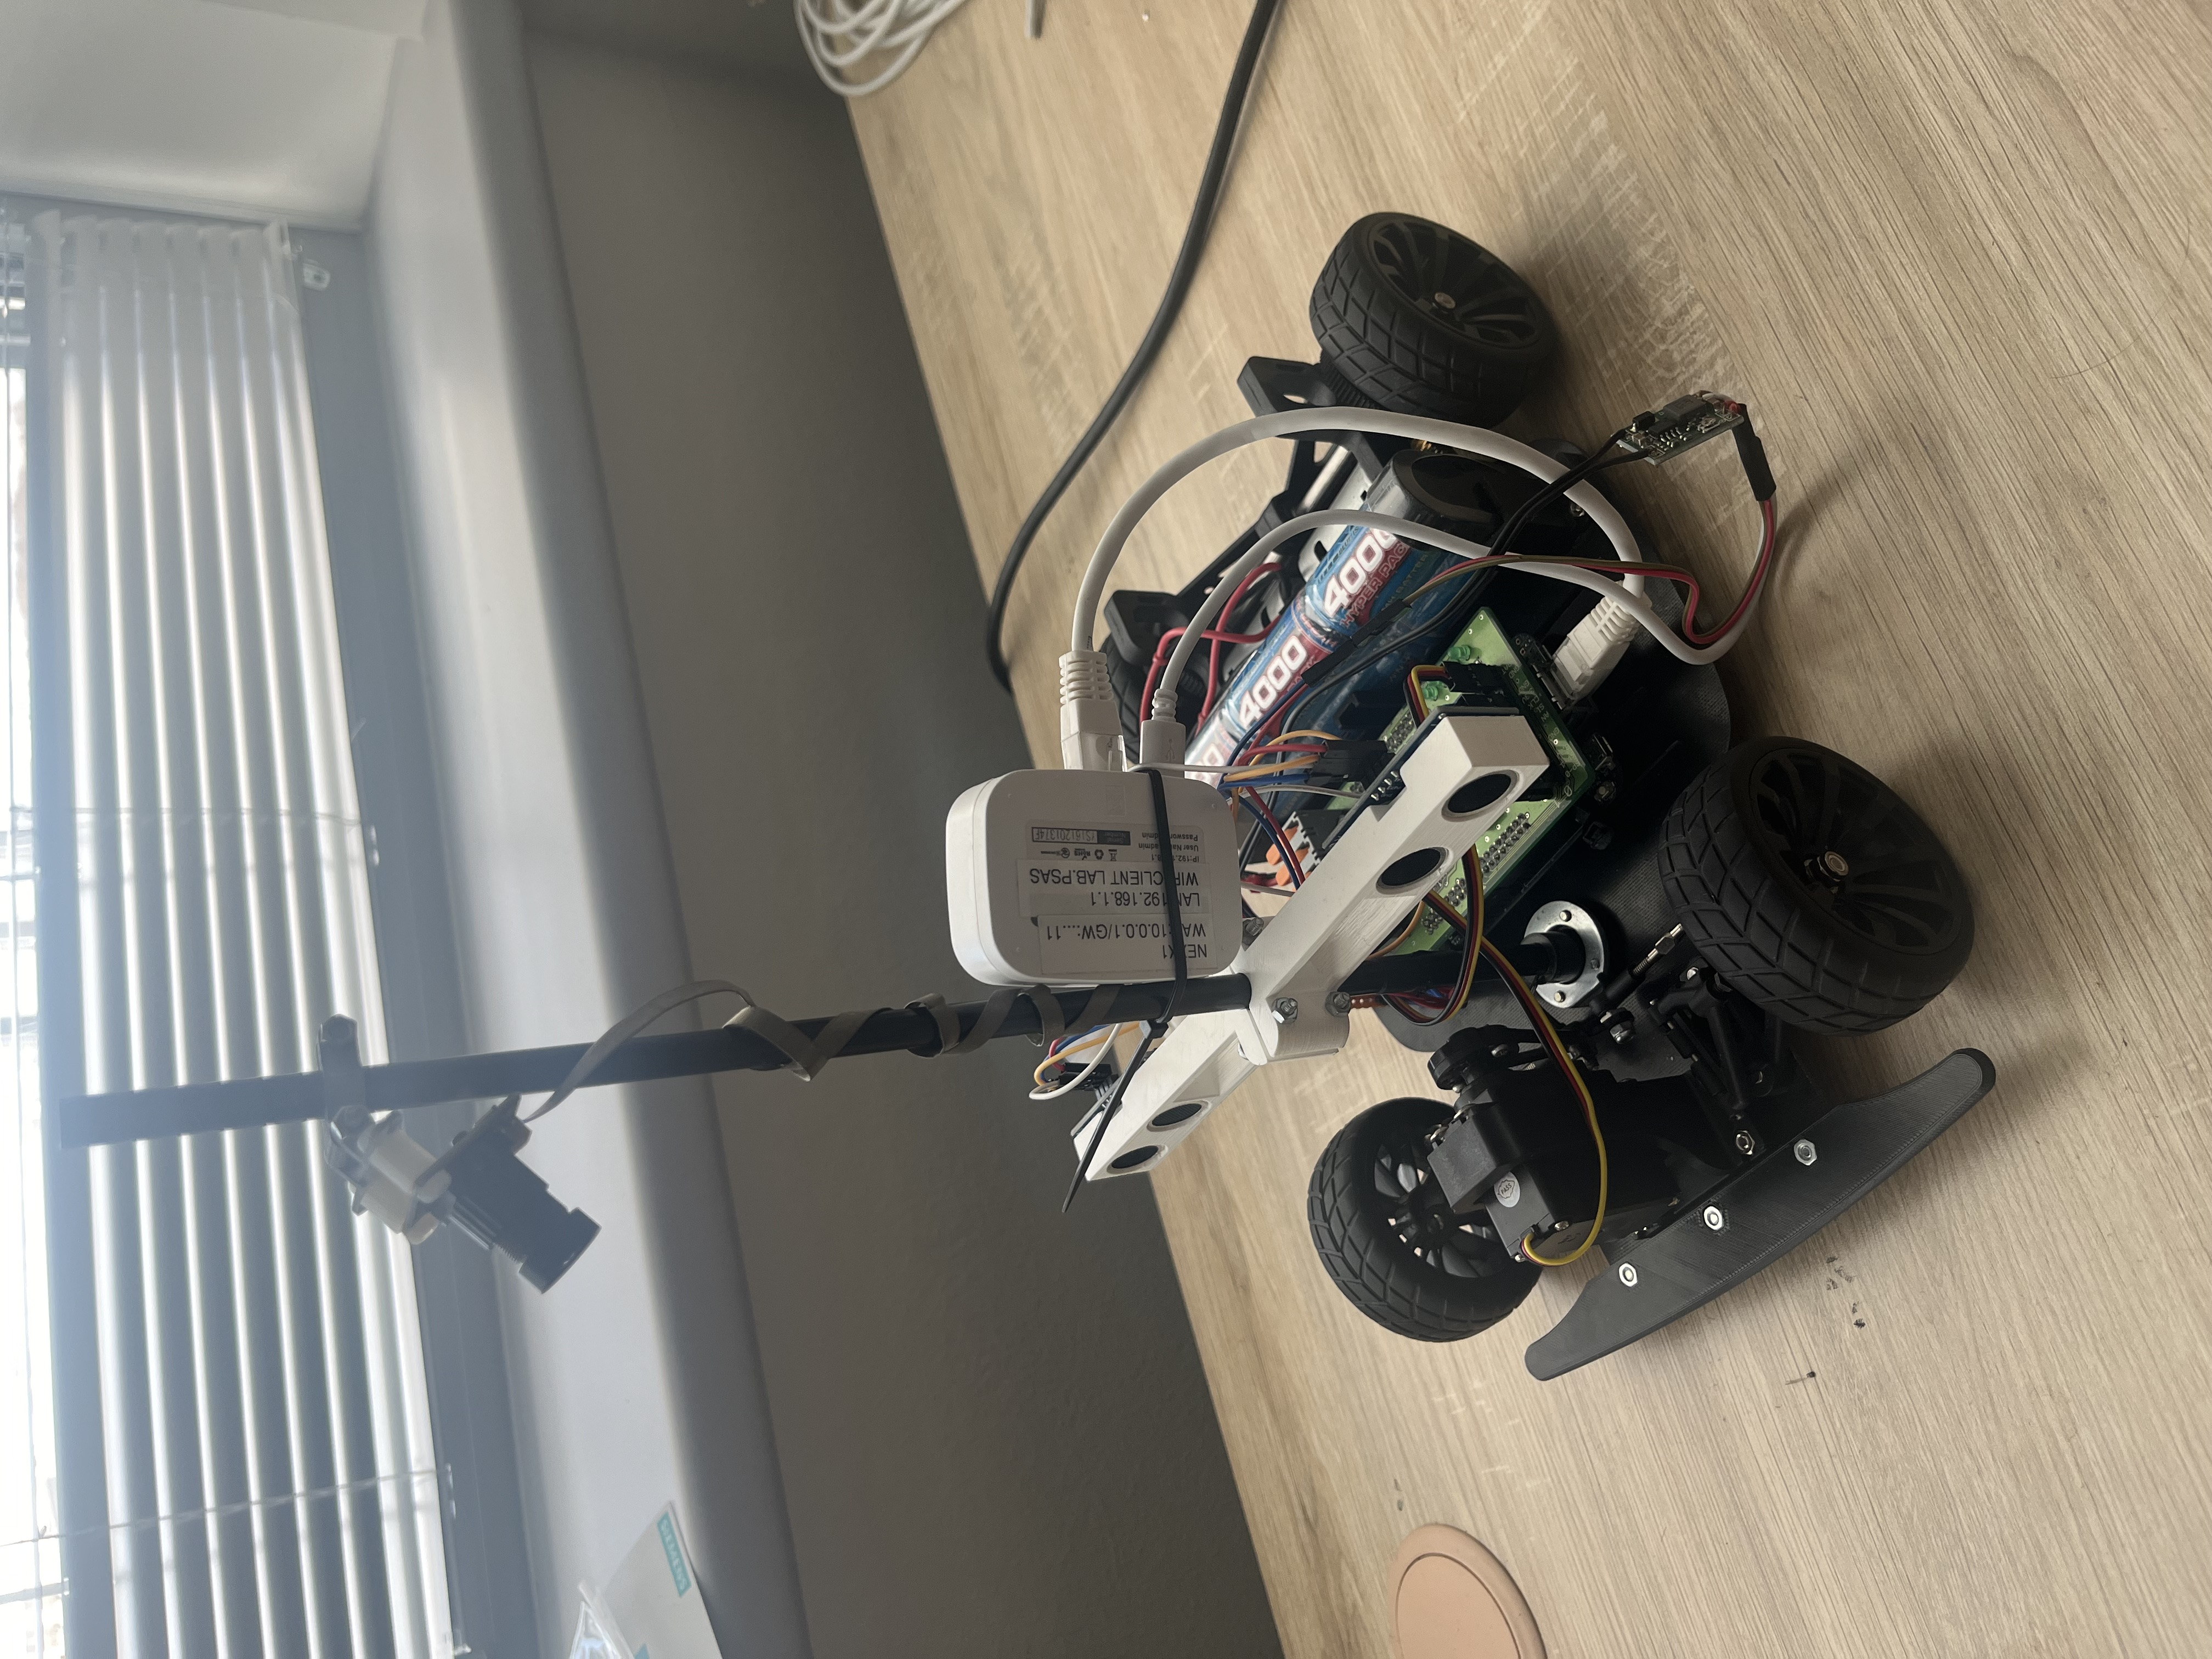
\includegraphics[width=0.45\linewidth, angle=-90]{Figures/car.jpeg}
    \caption{Model auta}
    \label{fig:car}
\end{figure}

\section{FRDM-K66F}
\label{sec:FRDM-K66F}\

FRDM-K66F je vývojová platforma od společnosti NXP určená pro MCU řady Kinetis K66 a K26.
Platforma je založena na jádře ARM© Cortex®-M4 a
konkrétně využívá model MK66FN2M0VMD18 s frekvencí 180 MHz, 2 MB flash paměti a 256 KB RAM.

Pro konektivitu platforma nabízí 2 micro-B USB porty, 1 ethernetový port a 54 GPIO konektorů.
GPIO piny jsou kompatibilní s Arduino™ R3, což poskytuje širokou škálu možností pro rozšiřující desky.
Pro další možnosti konektivity je deska vybavena moduly Bluetooth a RF.

Pro ladění je na platformě přítomno rozhraní OpenSDAv2.1, které podporuje J-Link.

Další užitečné periferie na desce zahrnují trojbarevnou LED, SDHC a digitální MEMS mikrofon.

Jako jednotku IMU platforma využívá akcelerometr společně s magnetometrem FXOS8700CQ
a gyroskop FXAS21002. Detailní popis jednotky je uveden v kapitole \ref{sec:IMU}.\cite{frdmk66UserGuide}

Vývojová platforma je znázorněna na obrázku \ref{fig:FRDM-K66F}.
\begin{figure}[h]
    \centering
    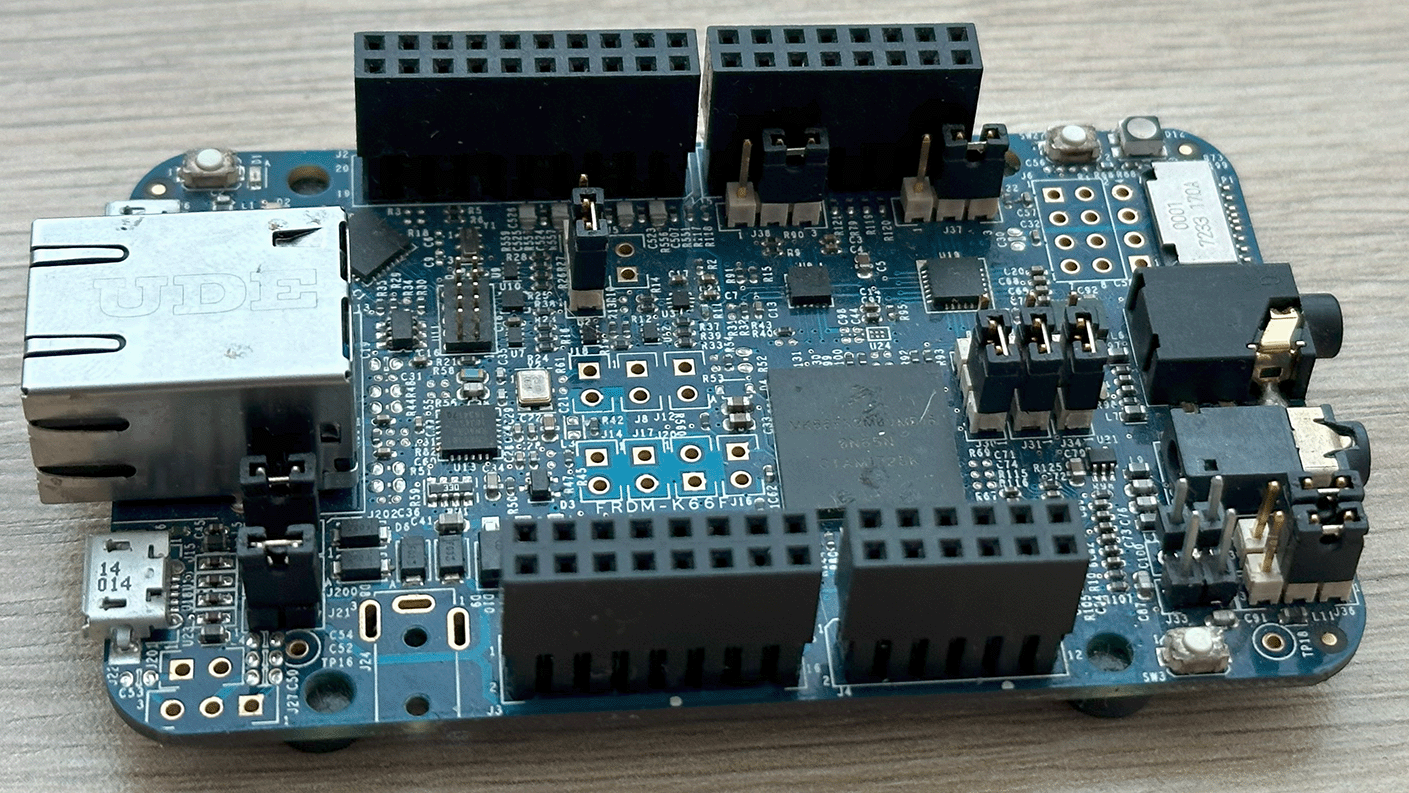
\includegraphics[width=0.45\linewidth]{Figures/FRDM-K66F.png}
    \caption{FRDM-K66F}
    \label{fig:FRDM-K66F}
\end{figure}

\section{POLI-TFC}
\label{sec:POLI-TFC}\

POLI-TFC shield je rozšiřující deska pro FRDM-K66F, která sjednocuje rozhraní pro
připojení periferií k vývojové desky. Shield obsahuje 2 konektoru pro PWM motory, 2 servomotoru,
2 rozhraní pro připojení řádkových kamer, 2 potenciometry, 4 DIP přepínače a 4 LED diody.
Shield je zobrazen na obrazku \ref{fig:POLI-TFC}.
\begin{figure}[h]
    \centering
    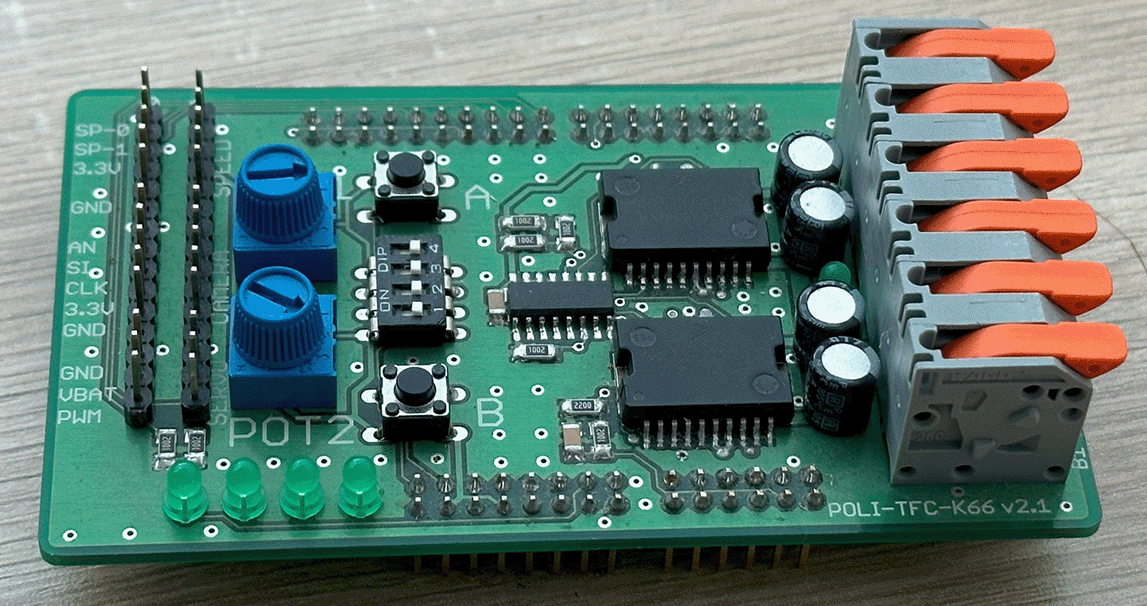
\includegraphics[width=0.45\linewidth]{Figures/POLI-TFC.png}
    \caption{POLI-TFC}
    \label{fig:POLI-TFC}
\end{figure}

\section{IMU}
\label{sec:IMU}\
V dnešní době jsou inerciální měřicí jednotky (IMU)
nezbytnou součástí mnoha technologických aplikací,
od mobilních telefonů a herních ovladačů až po pokročilé robotické systémy
a autonomní vozidla. IMU poskytují cenné informace o pohybu
a orientaci zařízení v prostoru, což umožňuje vývojářům implementovat
sofistikované funkce jako je navigace, sledování pohybu, stabilizace obrazu a mnoho dalších.

Deska FRDM-K66F obsahuje dva komponentů IMU jednotky - FXOS8700CQ a FXAS21002.\cite{frdmk66UserGuide}

\subsection{FXOS8700CQ}\

FXOS8700CQ je pokročilý 6-osý senzor, který kombinuje funkce 3-osého akcelerometru
a 3-osého magnetometru do jednoho čipu. Akcelerometr v senzoru FXOS8700CQ má
nastavitelné rozsahy ±2 g, ±4 g, ±8 g s 14-bitovým rozlišením, zatímco magnetometr
poskytuje 16-bitové rozlišení s rozsahem ±1200 µT na osu. Pro komunikaci podporuje
I2C a SPI rozhraní. Má dva piny pro přerušení a podporuje odesílat data rychlosti
až 800 Hz pro každý senzor a až 400 Hz v hybridnim režimu.
Tato integrace umožňuje zařízení zachytit komplexní data o svém pohybu a
orientaci vůči zemskému gravitačnímu a magnetickému poli.\cite{FXOS8700CQ}

\subsection{FXAS21002}\

FXAS21002 je vysoce výkonný 3-osy senzor, který poskytuje data o úhlové rychlosti
zrychlení. Tento senzor má nastavitelné rozsahy ±250, ±500, ±1000, a ±2000 stupňů za sekundu
s 16-bitovým rozlišením. Pro komunikaci podporuje I2C a SPI rozhraní.
Má dva piny pro přerušení a podporuje odesílat data rychlosti až 800 Hz.
To umožňuje zařízení detekovat rotace kolem svych os.\cite{FXAS21002}

\endinput
